\documentclass{beamer}
\let\Tiny=\tiny %to avoid warnings related to font size and beamer 
\usepackage{../beamerthemeAmsterdam}
%\usetheme{Amsterdam}
\usecolortheme{dolphin}

\usepackage{color}

\let\oldfootnotesize\footnotesize
\renewcommand*{\footnotesize}{\oldfootnotesize\tiny}

\newcommand\fG[1]{\textcolor{green!80!black}{#1}}
\newcommand\fR[1]{\textcolor{red!80!black}{#1}}


\title{Topic 3: Cloud Computing}
\author{Soodeh Farokhi, Gajo Gajic, Martin Kalany and Jia Wei}
\date{\today}

\begin{document}
\frame{\titlepage}

\begin{frame}
\frametitle{The task}

Develope a cloud-based service for twitter-based sentiment analysis on top of
\begin{itemize}
\item an IaaS environment (Amazon Web Services) using CloudScale
\item and a PaaS environment (Google AppEngine)
\end{itemize}

and compare this two cloud computing approaches.

\end{frame}


\begin{frame}
\frametitle{Google AppEngine: Architecture}
\begin{figure}
 \centerline{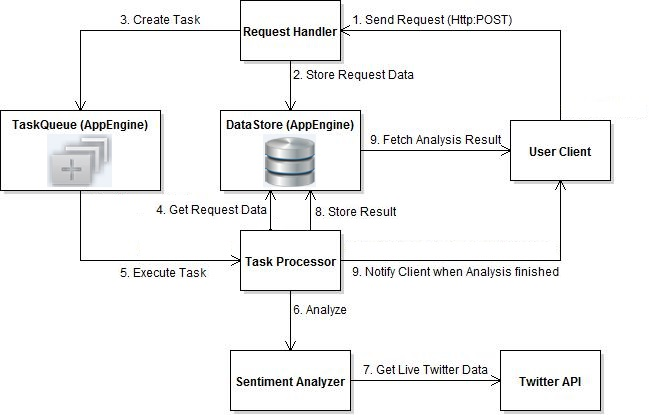
\includegraphics[width=1\columnwidth]{AppEngine.png}}
  \label{fig:appengine}
\end{figure}
\end{frame}
  
\begin{frame}
\frametitle{AWS + CloudScale: Architecture}
\end{frame}

\begin{frame}
\frametitle{CloudScale vs. Google AppEngine}
A CloudScale app
\begin{itemize}
\item is a \fG{simple Java SE program}
\item with \fG{a few annotations} plus a \fG{configuration} class,
\item more flexibility due to custom \fG{scaling} strategies
\item and \fG{no constraints on thread execution time}. 
\item \fR{Documentation} is (comparatively) \fR{scarce}
\item and the configuration quite \fR{tedious}.
\item \fR{Google} provides a \fR{vast and helpful ecosystem}.
\end{itemize}
\end{frame}

\begin{frame}
\fR{Questions?} \fG{Answers!}
\end{frame}

\end{document}